\chapter{Примеры оформления элементов}

\section{Примеры рисунков}

\subsection{Простой рисунок}

\begin{figure}[H]
\centering
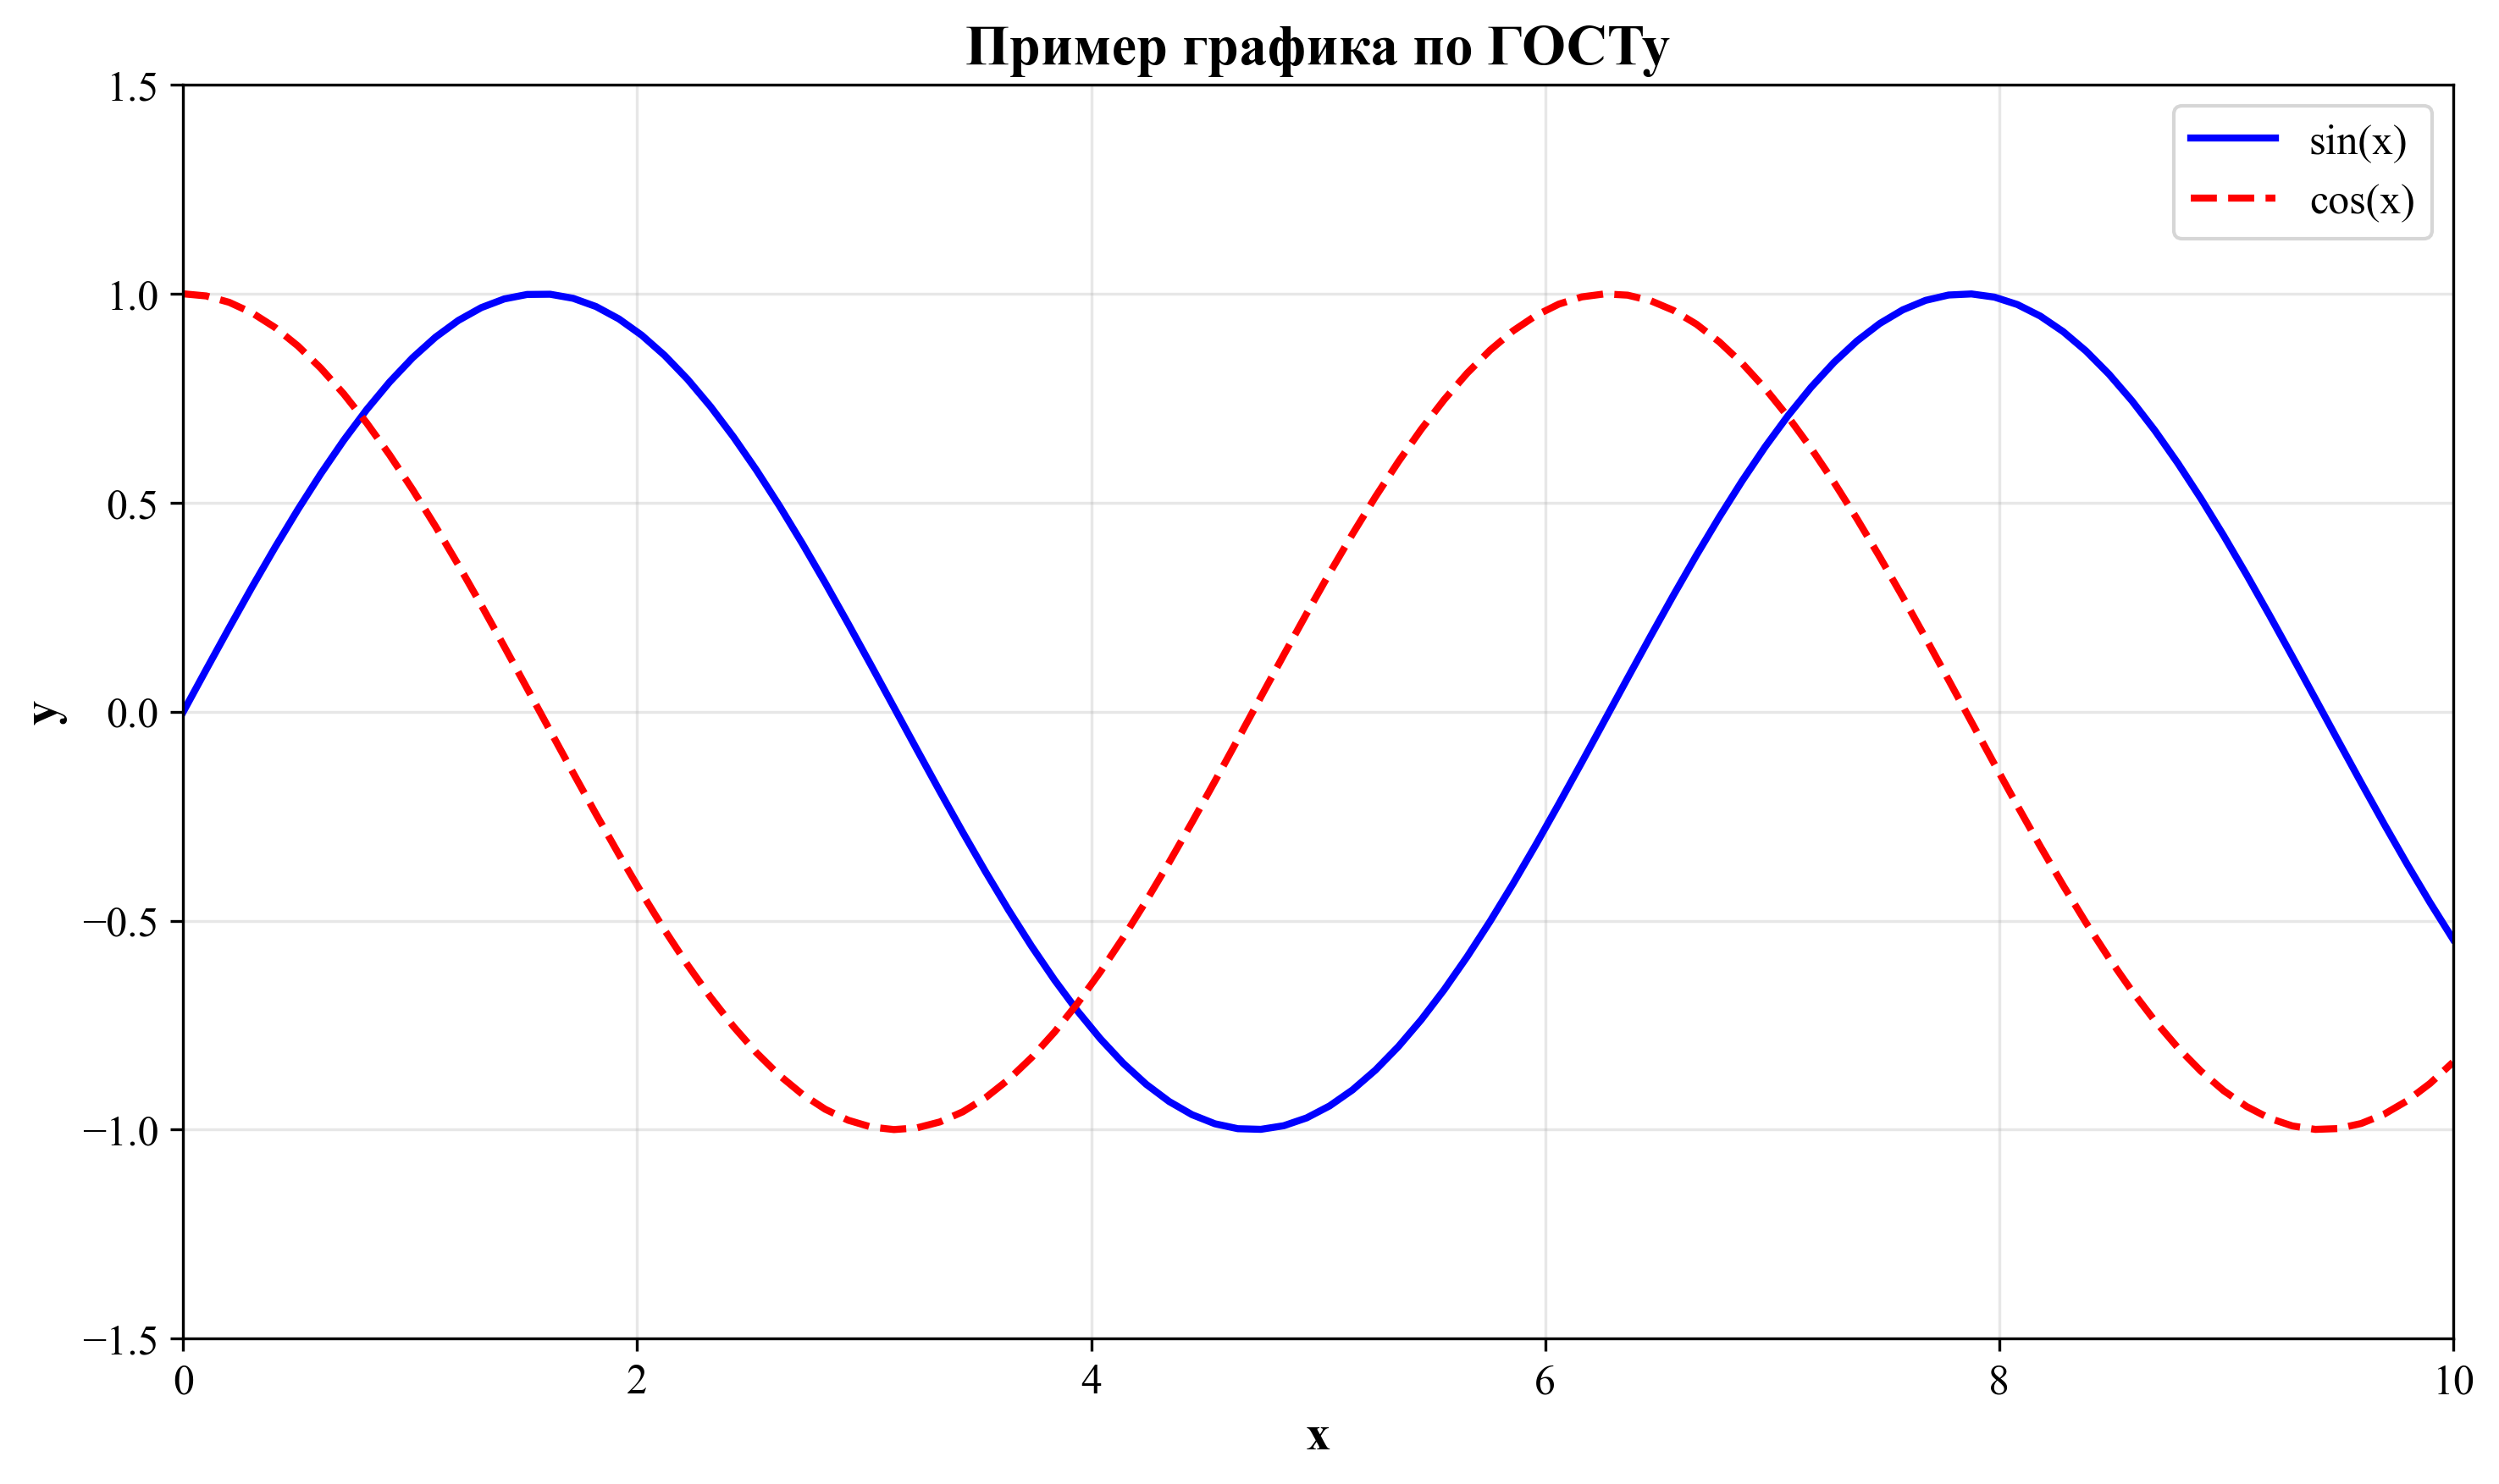
\includegraphics[width=0.8\textwidth]{images/example_plot.png}
\caption{Пример графика результатов эксперимента}
\label{fig:example_plot}
\end{figure}

Как показано на рисунке \ref{fig:example_plot}, результаты эксперимента демонстрируют...

\section{Примеры таблиц}

\subsection{Простая таблица}

\begin{table}[H]
\centering
\caption{Статистические данные}
\label{tab:statistics}
\begin{tabular}{|l|c|c|}
\hline
\textbf{Параметр} & \textbf{Значение} & \textbf{Единица} \\
\hline
Среднее & 15.6 & мм \\
Стандартное отклонение & 2.3 & мм \\
Минимум & 12.1 & мм \\
Максимум & 18.9 & мм \\
\hline
\end{tabular}
\end{table}

Данные представлены в таблице \ref{tab:statistics}.

\subsection{Длинная таблица с переносом}

\begin{longtable}{|c|l|c|c|}
\caption{Результаты экспериментов} \label{tab:long_experiments} \\

\hline
\textbf{№} & \textbf{Образец} & \textbf{Параметр 1} & \textbf{Параметр 2} \\
\hline
\endfirsthead

\tablecontinuation{\thetable} \\
\hline
\textbf{№} & \textbf{Образец} & \textbf{Параметр 1} & \textbf{Параметр 2} \\
\hline
\endhead

\hline
\endfoot

\hline
\endlastfoot

1 & A1 & 0.1 & 0.95 \\
2 & A2 & 0.2 & 0.87 \\
3 & A3 & 0.3 & 0.92 \\
4 & B1 & 0.4 & 0.88 \\
5 & B2 & 0.5 & 0.91 \\
6 & B3 & 0.6 & 0.89 \\
7 & C1 & 0.7 & 0.93 \\
8 & C2 & 0.8 & 0.86 \\
9 & C3 & 0.9 & 0.94 \\
10 & D1 & 1.0 & 0.90 \\
11 & A1 & 0.1 & 0.95 \\
12 & A2 & 0.2 & 0.87 \\
13 & A3 & 0.3 & 0.92 \\
14 & B1 & 0.4 & 0.88 \\
15 & B2 & 0.5 & 0.91 \\
16 & B3 & 0.6 & 0.89 \\
17 & C1 & 0.7 & 0.93 \\
18 & C2 & 0.8 & 0.86 \\
19 & C3 & 0.9 & 0.94 \\
20 & D1 & 1.0 & 0.90 \\
21 & A1 & 0.1 & 0.95 \\
22 & A2 & 0.2 & 0.87 \\
23 & A3 & 0.3 & 0.92 \\
24 & B1 & 0.4 & 0.88 \\
25 & B2 & 0.5 & 0.91 \\
26 & B3 & 0.6 & 0.89 \\
27 & C1 & 0.7 & 0.93 \\
28 & C2 & 0.8 & 0.86 \\
29 & C3 & 0.9 & 0.94 \\
30 & D1 & 1.0 & 0.90 \\
31 & A1 & 0.1 & 0.95 \\
32 & A2 & 0.2 & 0.87 \\
33 & A3 & 0.3 & 0.92 \\
34 & B1 & 0.4 & 0.88 \\
35 & B2 & 0.5 & 0.91 \\
36 & B3 & 0.6 & 0.89 \\
37 & C1 & 0.7 & 0.93 \\
38 & C2 & 0.8 & 0.86 \\
39 & C3 & 0.9 & 0.94 \\
40 & D1 & 1.0 & 0.90 \\
41 & A1 & 0.1 & 0.95 \\
42 & A2 & 0.2 & 0.87 \\
43 & A3 & 0.3 & 0.92 \\
44 & B1 & 0.4 & 0.88 \\
45 & B2 & 0.5 & 0.91 \\
46 & B3 & 0.6 & 0.89 \\
47 & C1 & 0.7 & 0.93 \\
48 & C2 & 0.8 & 0.86 \\
49 & C3 & 0.9 & 0.94 \\
50 & D1 & 1.0 & 0.90 \\
\end{longtable}

\section{Примеры листингов кода}

\subsection{Простой листинг}

\begin{lstlisting}[language=Python, caption={Пример простого алгоритма}, label={lst:simple_algorithm}]
def calculate_sum(a, b):
    """Calculate sum of two numbers"""
    return a + b

# Example usage
result = calculate_sum(5, 3)
print(f"Sum: {result}")
\end{lstlisting}

\subsection{Ультимативный способ описания кода}

\begin{lstlisting}[style=code, language=Python, caption={Пример Python кода с улучшенной подсветкой}, label={lst:python_enhanced}]
def calculate_sum(a, b):
    """Calculate sum of two numbers"""
    return a + b

# Example usage
result = calculate_sum(5, 3)
print(f"Sum: {result}")
\end{lstlisting}

\subsection{Листинг с улучшенным переносом (fvextra)}

\begin{CodeBreakable}
def calculate_sum(a, b):
    """Calculate sum of two numbers"""
    return a + b

# Example usage
result = calculate_sum(5, 3)
print(f"Sum: {result}")
\end{CodeBreakable}

\subsection{Длинный листинг с переносом}

\begin{lstlisting}[style=code, language=Python, caption={Пример алгоритма машинного обучения с улучшенной подсветкой}, label={lst:ml_algorithm_enhanced}]
import numpy as np
import pandas as pd
from sklearn.model_selection import train_test_split, cross_val_score
from sklearn.ensemble import RandomForestClassifier, GradientBoostingClassifier
from sklearn.svm import SVC
from sklearn.metrics import accuracy_score, classification_report
import matplotlib.pyplot as plt
import seaborn as sns

def load_data(filepath):
    """Load and preprocess data"""
    data = pd.read_csv(filepath)
    
    # Handle missing values
    data = data.fillna(data.mean())
    
    # Encode categorical variables
    categorical_columns = data.select_dtypes(include=['object']).columns
    for col in categorical_columns:
        data[col] = pd.Categorical(data[col]).codes
    
    return data

def train_model(X_train, y_train, model_type='random_forest'):
    """Train machine learning model"""
    if model_type == 'random_forest':
        model = RandomForestClassifier(n_estimators=100, random_state=42)
    elif model_type == 'gradient_boosting':
        model = GradientBoostingClassifier(n_estimators=100, random_state=42)
    elif model_type == 'svm':
        model = SVC(kernel='rbf', random_state=42)
    else:
        raise ValueError("Unknown model type")
    
    model.fit(X_train, y_train)
    return model

def evaluate_model(model, X_test, y_test, model_type):
    """Evaluate model performance"""
    y_pred = model.predict(X_test)
    accuracy = accuracy_score(y_test, y_pred)
    
    # Cross-validation
    cv_scores = cross_val_score(model, X_test, y_test, cv=5)
    
    # Print results
    print(f"Model: {model_type}")
    print(f"Accuracy: {accuracy:.4f}")
    print(f"CV Score: {cv_scores.mean():.4f} (+/- {cv_scores.std() * 2:.4f})")
    print("\nClassification Report:")
    print(classification_report(y_test, y_pred))
    
    return model, accuracy, y_pred

def plot_results(y_true, y_pred, model_name):
    """Plot classification results"""
    plt.figure(figsize=(10, 6))
    
    # Confusion matrix
    from sklearn.metrics import confusion_matrix
    cm = confusion_matrix(y_true, y_pred)
    
    plt.subplot(1, 2, 1)
    sns.heatmap(cm, annot=True, fmt='d', cmap='Blues')
    plt.title(f'Confusion Matrix - {model_name}')
    plt.xlabel('Predicted')
    plt.ylabel('Actual')
    
    # Feature importance (for tree-based models)
    plt.subplot(1, 2, 2)
    if hasattr(model, 'feature_importances_'):
        importances = model.feature_importances_
        indices = np.argsort(importances)[::-1][:10]
        plt.bar(range(10), importances[indices])
        plt.title(f'Feature Importance - {model_name}')
        plt.xlabel('Feature Index')
        plt.ylabel('Importance')
    
    plt.tight_layout()
    plt.show()

def main():
    """Main execution function"""
    # Load data
    data = load_data('data.csv')
    
    # Prepare features and target
    X = data.drop('target', axis=1)
    y = data['target']
    
    # Split data
    X_train, X_test, y_train, y_test = train_test_split(
        X, y, test_size=0.2, random_state=42
    )
    
    # Train and evaluate different models
    models = ['random_forest', 'gradient_boosting', 'svm']
    results = {}
    
    for model_type in models:
        print(f"\n=== Training {model_type} ===")
        model = train_model(X_train, y_train, model_type)
        model, accuracy, y_pred = evaluate_model(model, X_test, y_test, model_type)
        results[model_type] = {
            'model': model,
            'accuracy': accuracy,
            'predictions': y_pred
        }
    
    # Print summary
    print("\n=== Results Summary ===")
    for model_name, result in results.items():
        print(f"{model_name}: {result['accuracy']:.4f}")
    
    # Plot results for best model
    best_model = max(results.items(), key=lambda x: x[1]['accuracy'])
    print(f"\nBest model: {best_model[0]} with accuracy {best_model[1]['accuracy']:.4f}")

if __name__ == "__main__":
    main()
\end{lstlisting}

\subsection{Примеры с разными языками программирования}

\subsubsection{Java код}

\begin{lstlisting}[style=code, language=Java, caption={Пример Java класса}, label={lst:java_example}]
public class Calculator {
    private double result;
    
    public Calculator() {
        this.result = 0.0;
    }
    
    public double add(double a, double b) {
        result = a + b;
        return result;
    }
    
    public double multiply(double a, double b) {
        result = a * b;
        return result;
    }
    
    public double getResult() {
        return result;
    }
}
\end{lstlisting}

\subsubsection{C++ код}

\begin{lstlisting}[style=code, language=C++, caption={Пример C++ класса}, label={lst:cpp_example}]
#include <iostream>
#include <vector>

class Matrix {
private:
    std::vector<std::vector<double>> data;
    int rows, cols;
    
public:
    Matrix(int r, int c) : rows(r), cols(c) {
        data.resize(rows, std::vector<double>(cols, 0.0));
    }
    
    void setValue(int row, int col, double value) {
        if (row >= 0 && row < rows && col >= 0 && col < cols) {
            data[row][col] = value;
        }
    }
    
    double getValue(int row, int col) const {
        if (row >= 0 && row < rows && col >= 0 && col < cols) {
            return data[row][col];
        }
        return 0.0;
    }
    
    void print() const {
        for (int i = 0; i < rows; i++) {
            for (int j = 0; j < cols; j++) {
                std::cout << data[i][j] << " ";
            }
            std::cout << std::endl;
        }
    }
};
\end{lstlisting}

\section{Примеры примечаний}

\subsection{Одно примечание}

\note{Все эксперименты проводились при температуре 20±2°C и относительной влажности 50±5\%.}

\subsection{Несколько примечаний}

\notes{
\item Все измерения проводились с точностью до 0.01 мм
\item Использовалось оборудование с сертификатом калибровки
\item Результаты получены на основе 100 независимых измерений
\item Статистическая значимость p < 0.05
}

\section{Примеры формул}

\subsection{Простая формула}

\begin{equation}
E = mc^2
\label{eq:einstein}
\end{equation}

Согласно формуле \ref{eq:einstein} энергия пропорциональна массе.

\subsection{Система уравнений}

\begin{align}
\frac{\partial u}{\partial t} &= \alpha \frac{\partial^2 u}{\partial x^2} \label{eq:heat1} \\
u(0,t) &= u(L,t) = 0 \label{eq:heat2} \\
u(x,0) &= f(x) \label{eq:heat3}
\end{align}

Уравнения \ref{eq:heat1}--\ref{eq:heat3} описывают процесс теплопроводности.

\section{Примеры списков}

\subsection{Нумерованный список}

\begin{enumerate}
\item Загрузка данных из файла
\item Предварительная обработка данных
\item Разделение на обучающую и тестовую выборки
\item Обучение модели
\item Оценка качества модели
\item Интерпретация результатов
\end{enumerate}

\subsection{Маркированный список}

\begin{itemize}
\item Машинное обучение
\item Глубокое обучение
\item Обработка естественного языка
\item Компьютерное зрение
\item Рекомендательные системы
\end{itemize}

\subsection{Вложенный список}

\begin{enumerate}
\item Подготовка данных
    \begin{enumerate}
    \item Очистка данных
    \item Нормализация
    \item Кодирование категориальных переменных
    \end{enumerate}
\item Обучение модели
    \begin{enumerate}
    \item Выбор алгоритма
    \item Настройка гиперпараметров
    \item Валидация модели
    \end{enumerate}
\item Оценка результатов
    \begin{enumerate}
    \item Метрики качества
    \item Визуализация результатов
    \item Интерпретация
    \end{enumerate}
\end{enumerate}
